\documentclass{article}
\usepackage{amsmath}
\usepackage{amssymb}
\newcommand*{\qed}{\hfill\ensuremath{\blacksquare}}
\usepackage{graphicx}
\graphicspath{{.}}
\usepackage{hyperref}

\title{Computational Linear Algebra, Module 10}
\author{Maya Shende}
\date{Due: April 11th, 2018}

\begin{document}
\maketitle

\begin{enumerate}

%exercise 1
\item interval = $[0, 2\pi]$: \\
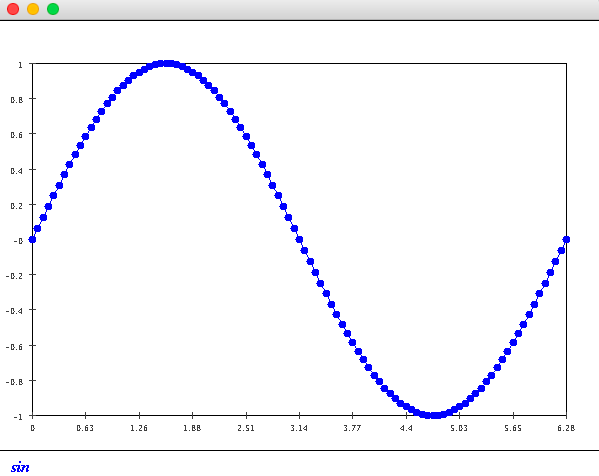
\includegraphics[scale=0.5]{exercise1_small_interval}\\
interval = $[0, 4\pi]$: \\
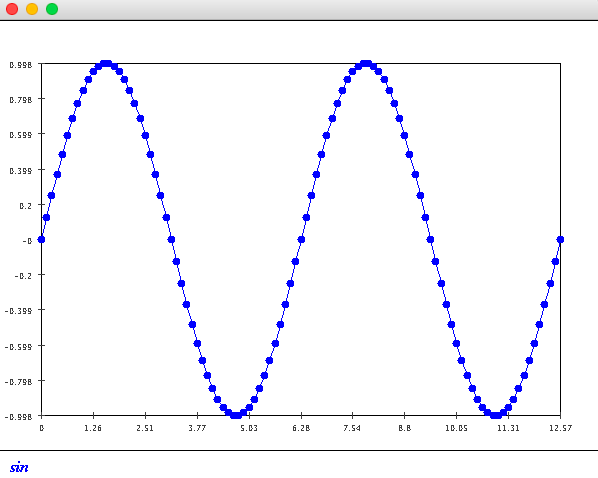
\includegraphics[scale=0.5]{exercise1_larger_interval}

%exercise 2
\item $n=1$:\\
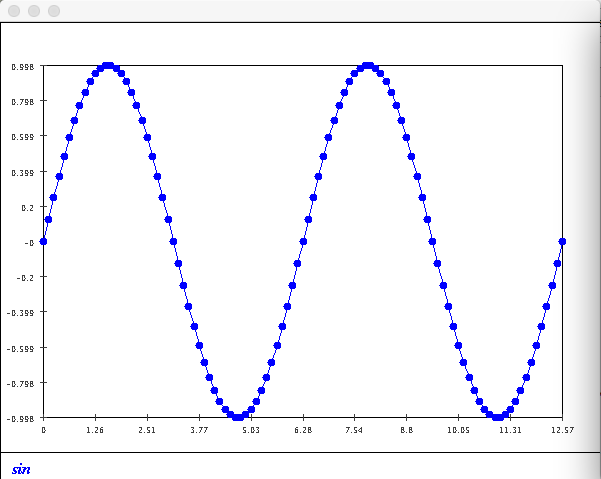
\includegraphics[scale=0.5]{exercise2_n1}\\
$n=2$: \\
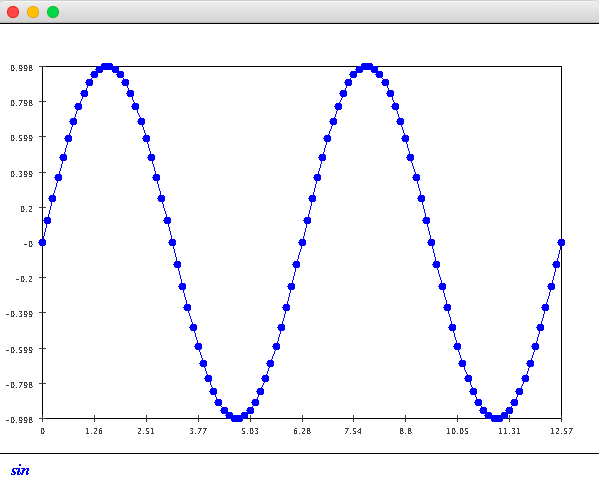
\includegraphics[scale=0.5]{exercise2_n2}\\
$n=3$:\\
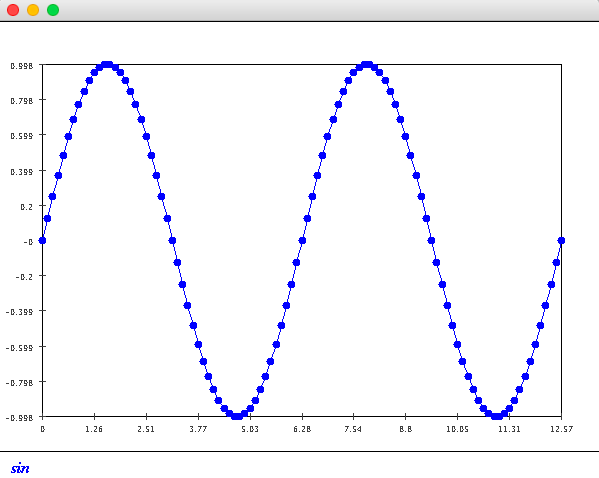
\includegraphics[scale=0.5]{exercise2_n3}

%exercise 3
\item $\tau=10$, $n=2$: \\
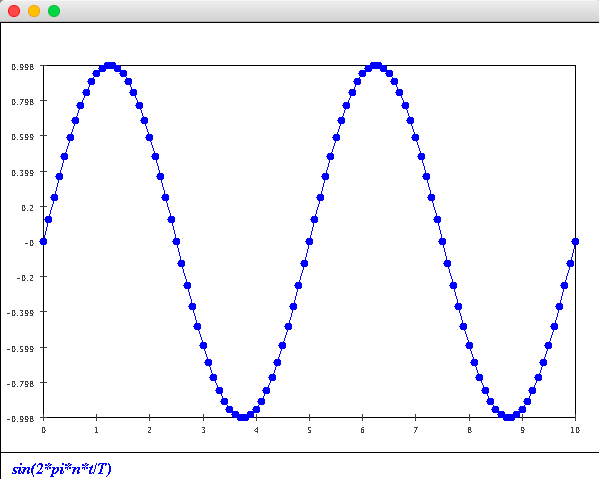
\includegraphics[scale=0.5]{exercise3_1}\\

$\tau=5$, $n=2$:\\
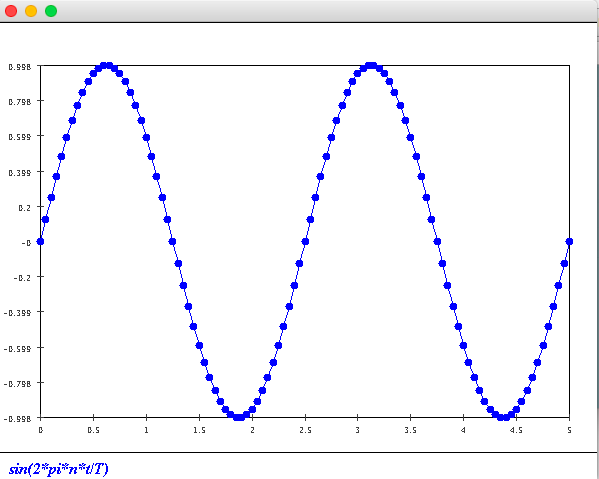
\includegraphics[scale=0.5]{exercise3_2}\\

$\tau=5$, $n=7$:\\
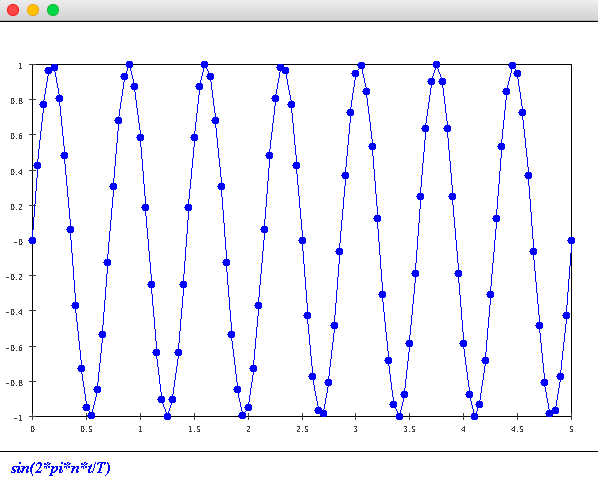
\includegraphics[scale=0.5]{exercise3_2_n-7}

%exercise 4
\item Mystery function: \\
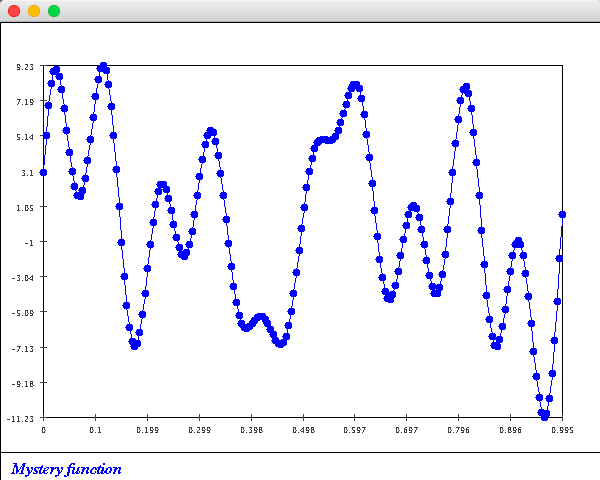
\includegraphics[scale=0.5]{exercise4}

%exercise 5
\item With high frequencies:\\
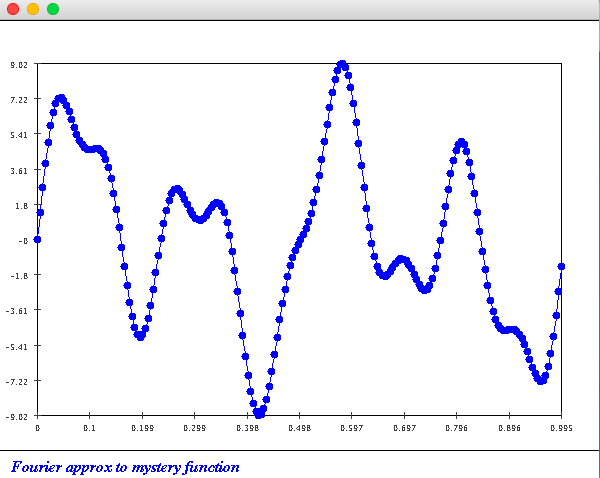
\includegraphics[scale=0.3]{exercise5_high}\\
Mystery function: \\
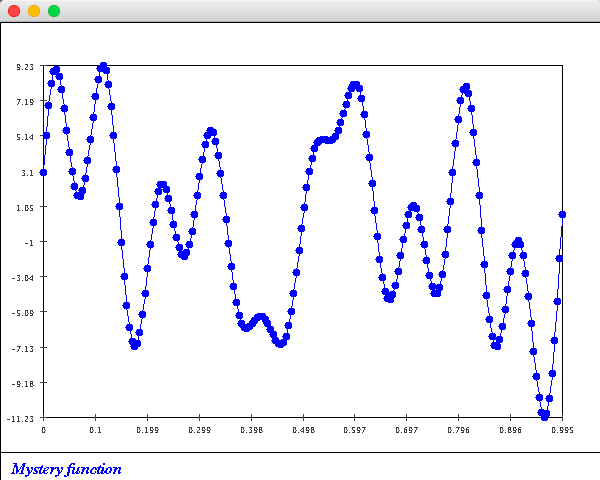
\includegraphics[scale=0.3]{exercise4}\\
Yes, this is a decent approximation of the mystery function, as long as the high frequencies are kept. 

%exercise 6
\item Without high frequencies: \\
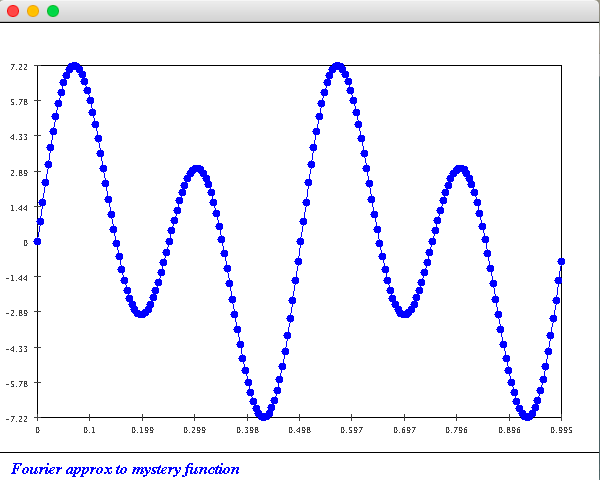
\includegraphics[scale=0.5]{exercise5_no_high}\\
This does capture the essence of the mystery function. \\

With $a[i] = 0$ for $i \geq 4$, the fourier sum no longer captures the essence of the mystery function because we lose too much of the high frequency information:\\
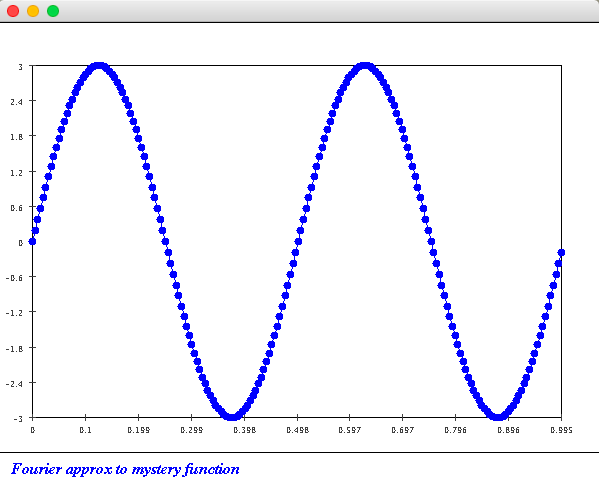
\includegraphics[scale=0.5]{exercise6}

%exercise 7
\item What I have so far:\\
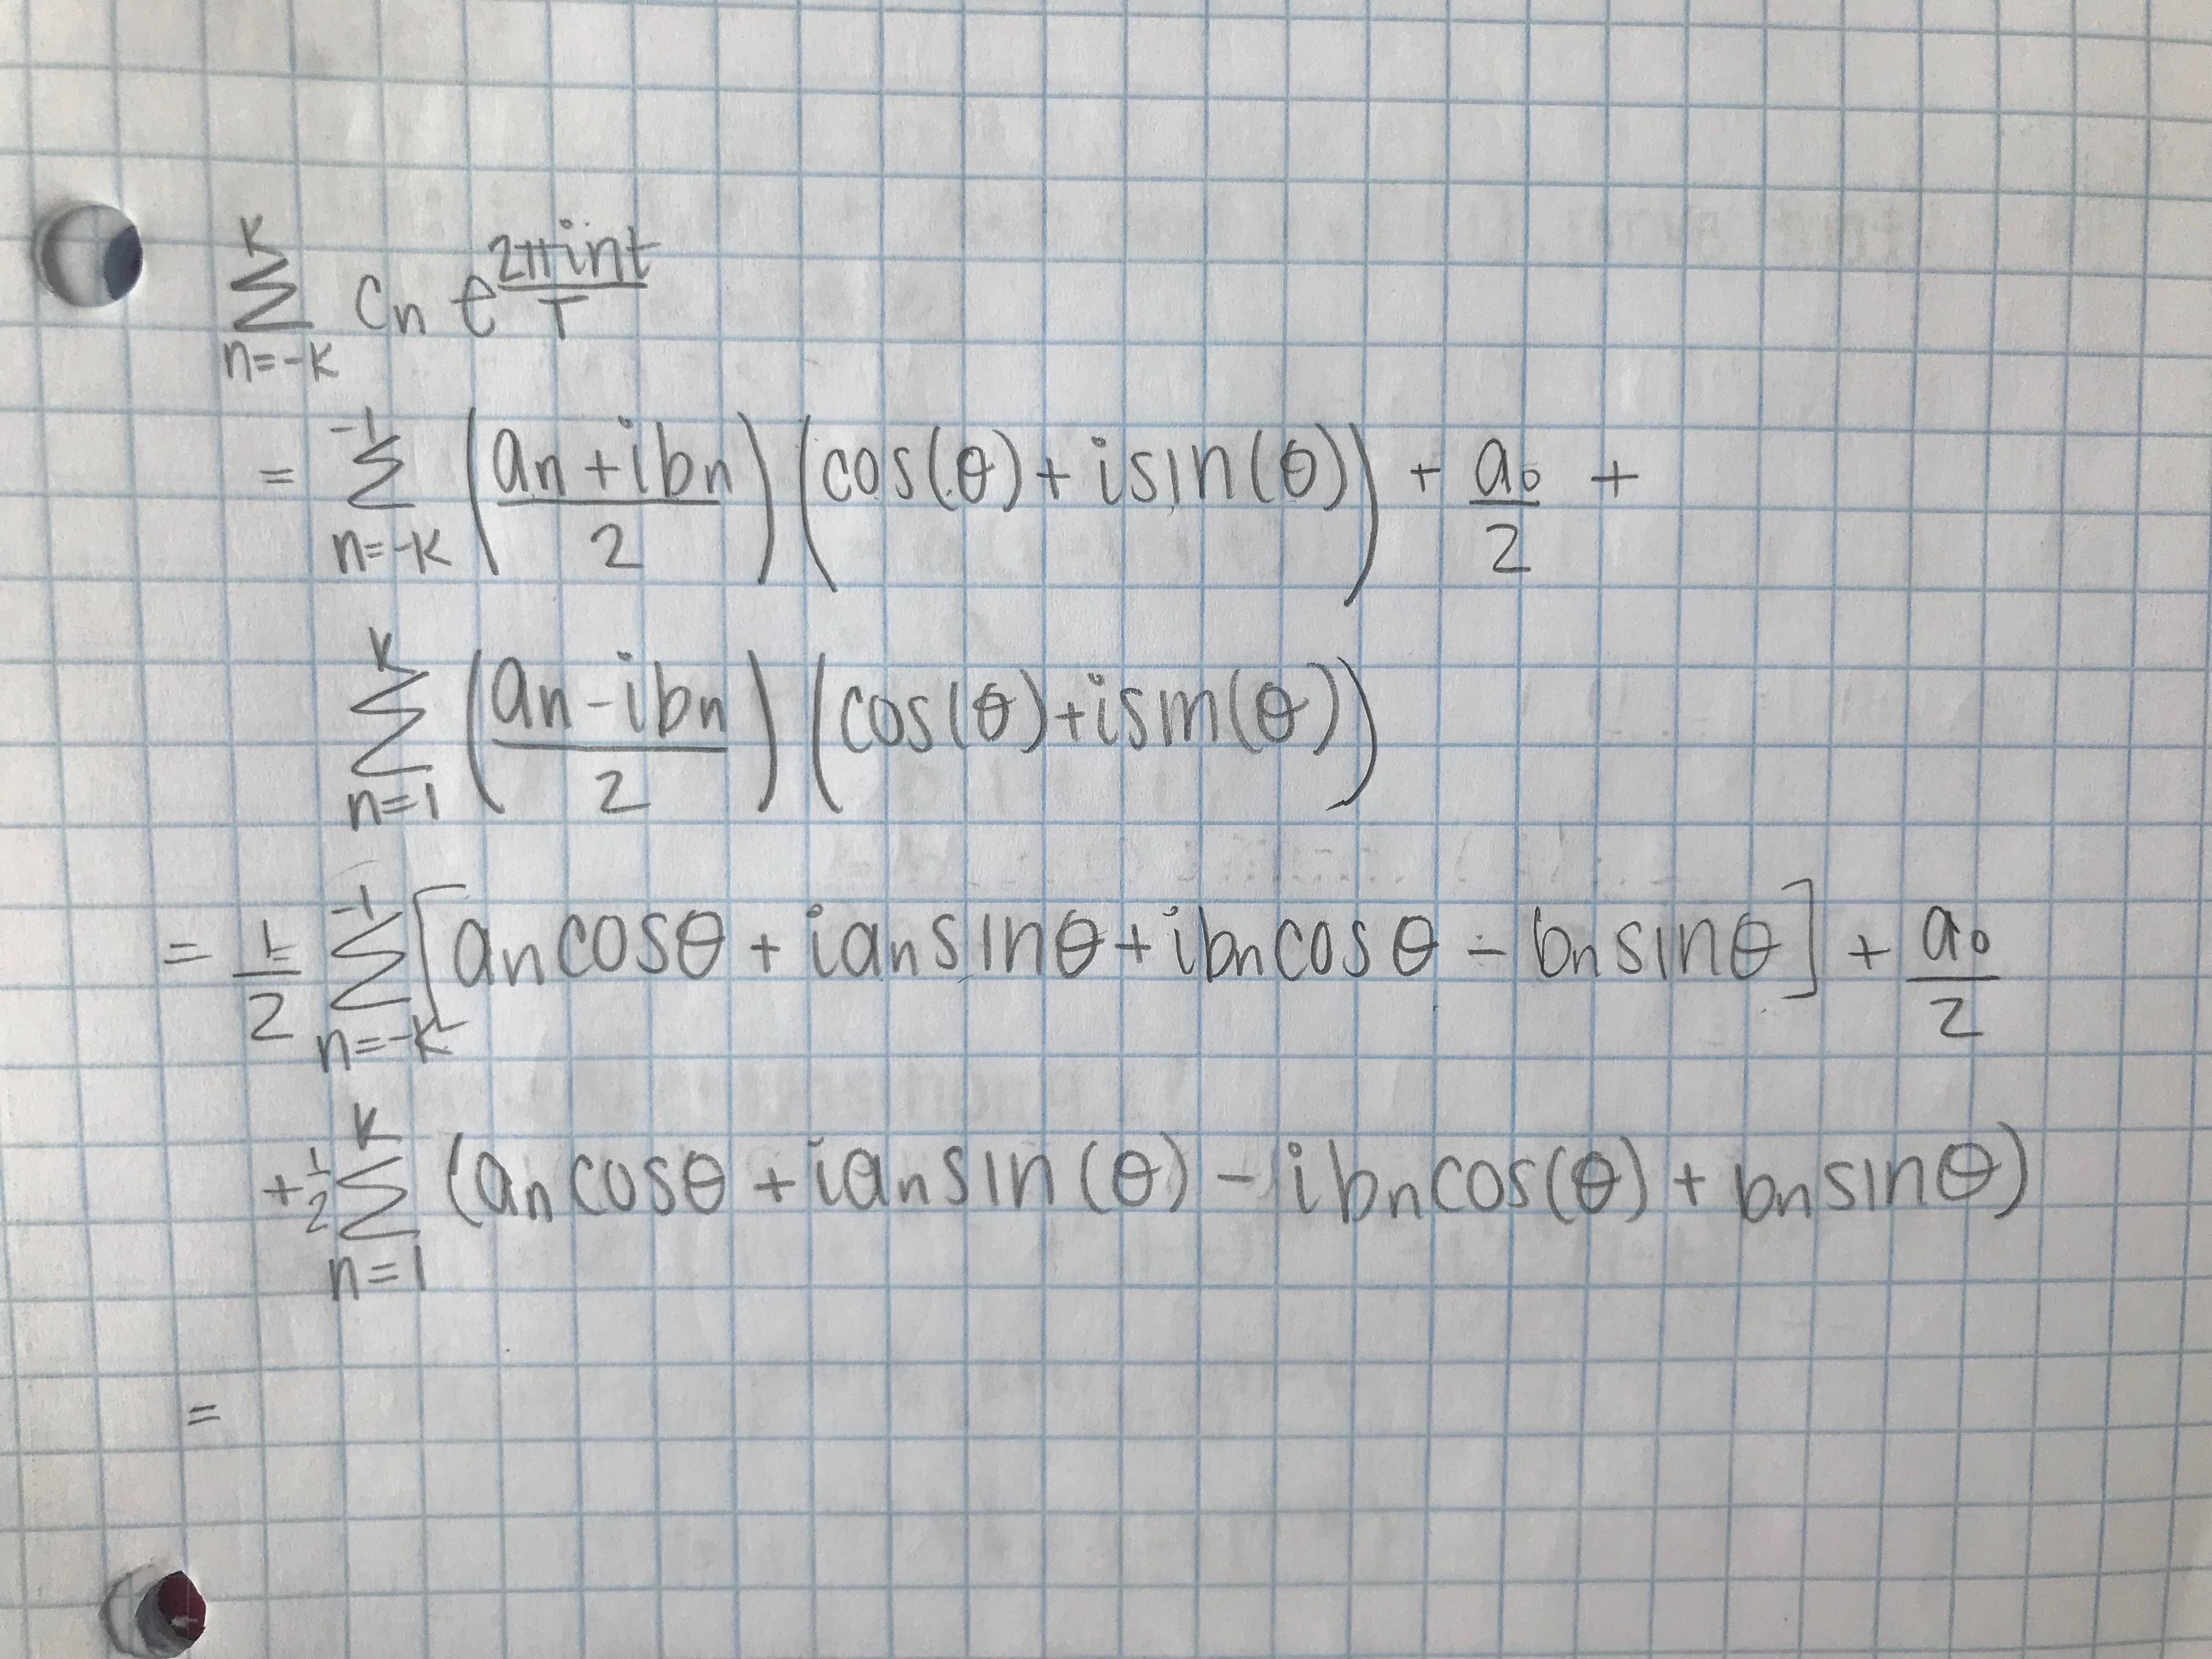
\includegraphics[scale=0.1]{exercise7}\\
I was not able to figure out how to get rid of the imaginary terms in this to get to what I am trying to show.

%exercise 8
\item This is true because for any value sof $p$ and $t$, we will always be adding a multiple of $2\pi$ to the first part of the sine, so that value of the sine will not change with or without this addition. 

%exercise 9
\item Plot:\\
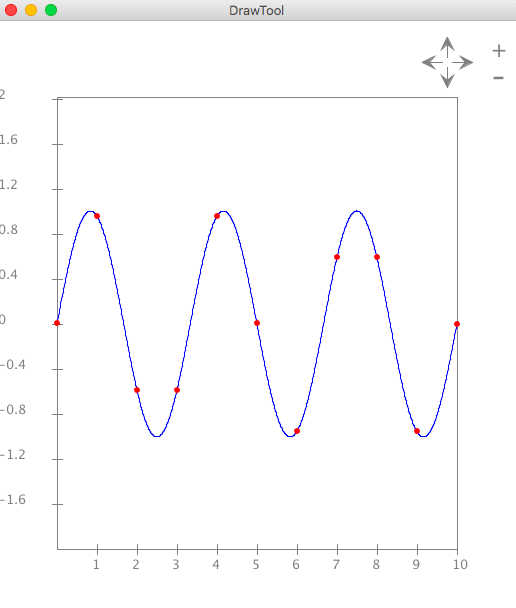
\includegraphics[scale=0.5]{exercise9}

%exercise 10
\item The points lie on both sine curves.

%exercise 11
\item 
\begin{eqnarray*}
f_3 &=& \sum_{n=0}^{3} F_nw^{3n}\\
&=& F_0w^0 + F_1w^3 + F_2w^6 + F_3w^9
\end{eqnarray*}

%exercise 12
\item For any number, you can span all other numbers, which is why it doesn't make sense to do a linear combination. The span of a single number by itself is the set of all $\mathbb{R}$.

%exercise 13
\item 
\begin{eqnarray*}
f_3 &=& \sum_{n=0}^{N-1} F_nw^{3n}\\
&=& F_0w^0 + F_1w^3 + F_2w^6 + \dots + F_{N-1}w^{3(N-1)}
\end{eqnarray*}

%exercise 14
\item $d_3 = 
\begin{bmatrix}
	1\\
	w^3\\
	w^6\\
	w^9\\
	\vdots\\
	w^{3(N-1)}
\end{bmatrix}
$

%exercise 15
\item The $4^{th}$ column is $d_3$. 

%exercise 16
\item There is a negative in front of the $q$ because we are doing the complex dot product, which involves using the conjugate of the second term in the multiplication, so we need to negate it. 
\begin{eqnarray*}
	s &=& 1 + z + z^2 + \dots + z{N+1}\\
	zs &=& z + z^2 + \dots + z^N\\
	zs - s &=& z + z^2 + \dots + z^N - (1 + z + z^2 + \dots + z{N+1})\\
	&=& z^N - 1\\
	s(z - 1) &=& z^N - 1\\
	s &=& \frac{z^N - 1}{z-1}
\end{eqnarray*}

%exercise 17
\item This is true because they are orthogonal.

%exercise 18
\item 
\begin{eqnarray*}
	w^N &=& \left(\exp^{\frac{2\pi i}{N}}\right)^N\\
	&=& \exp^{2 \pi i}\\
	&=& \cos{(2 \pi)} - i \sin{(2 \pi)}\\
	&=& 1 - 0\\
	&=& 1
\end{eqnarray*}

%exercise 19
\item plot: \\
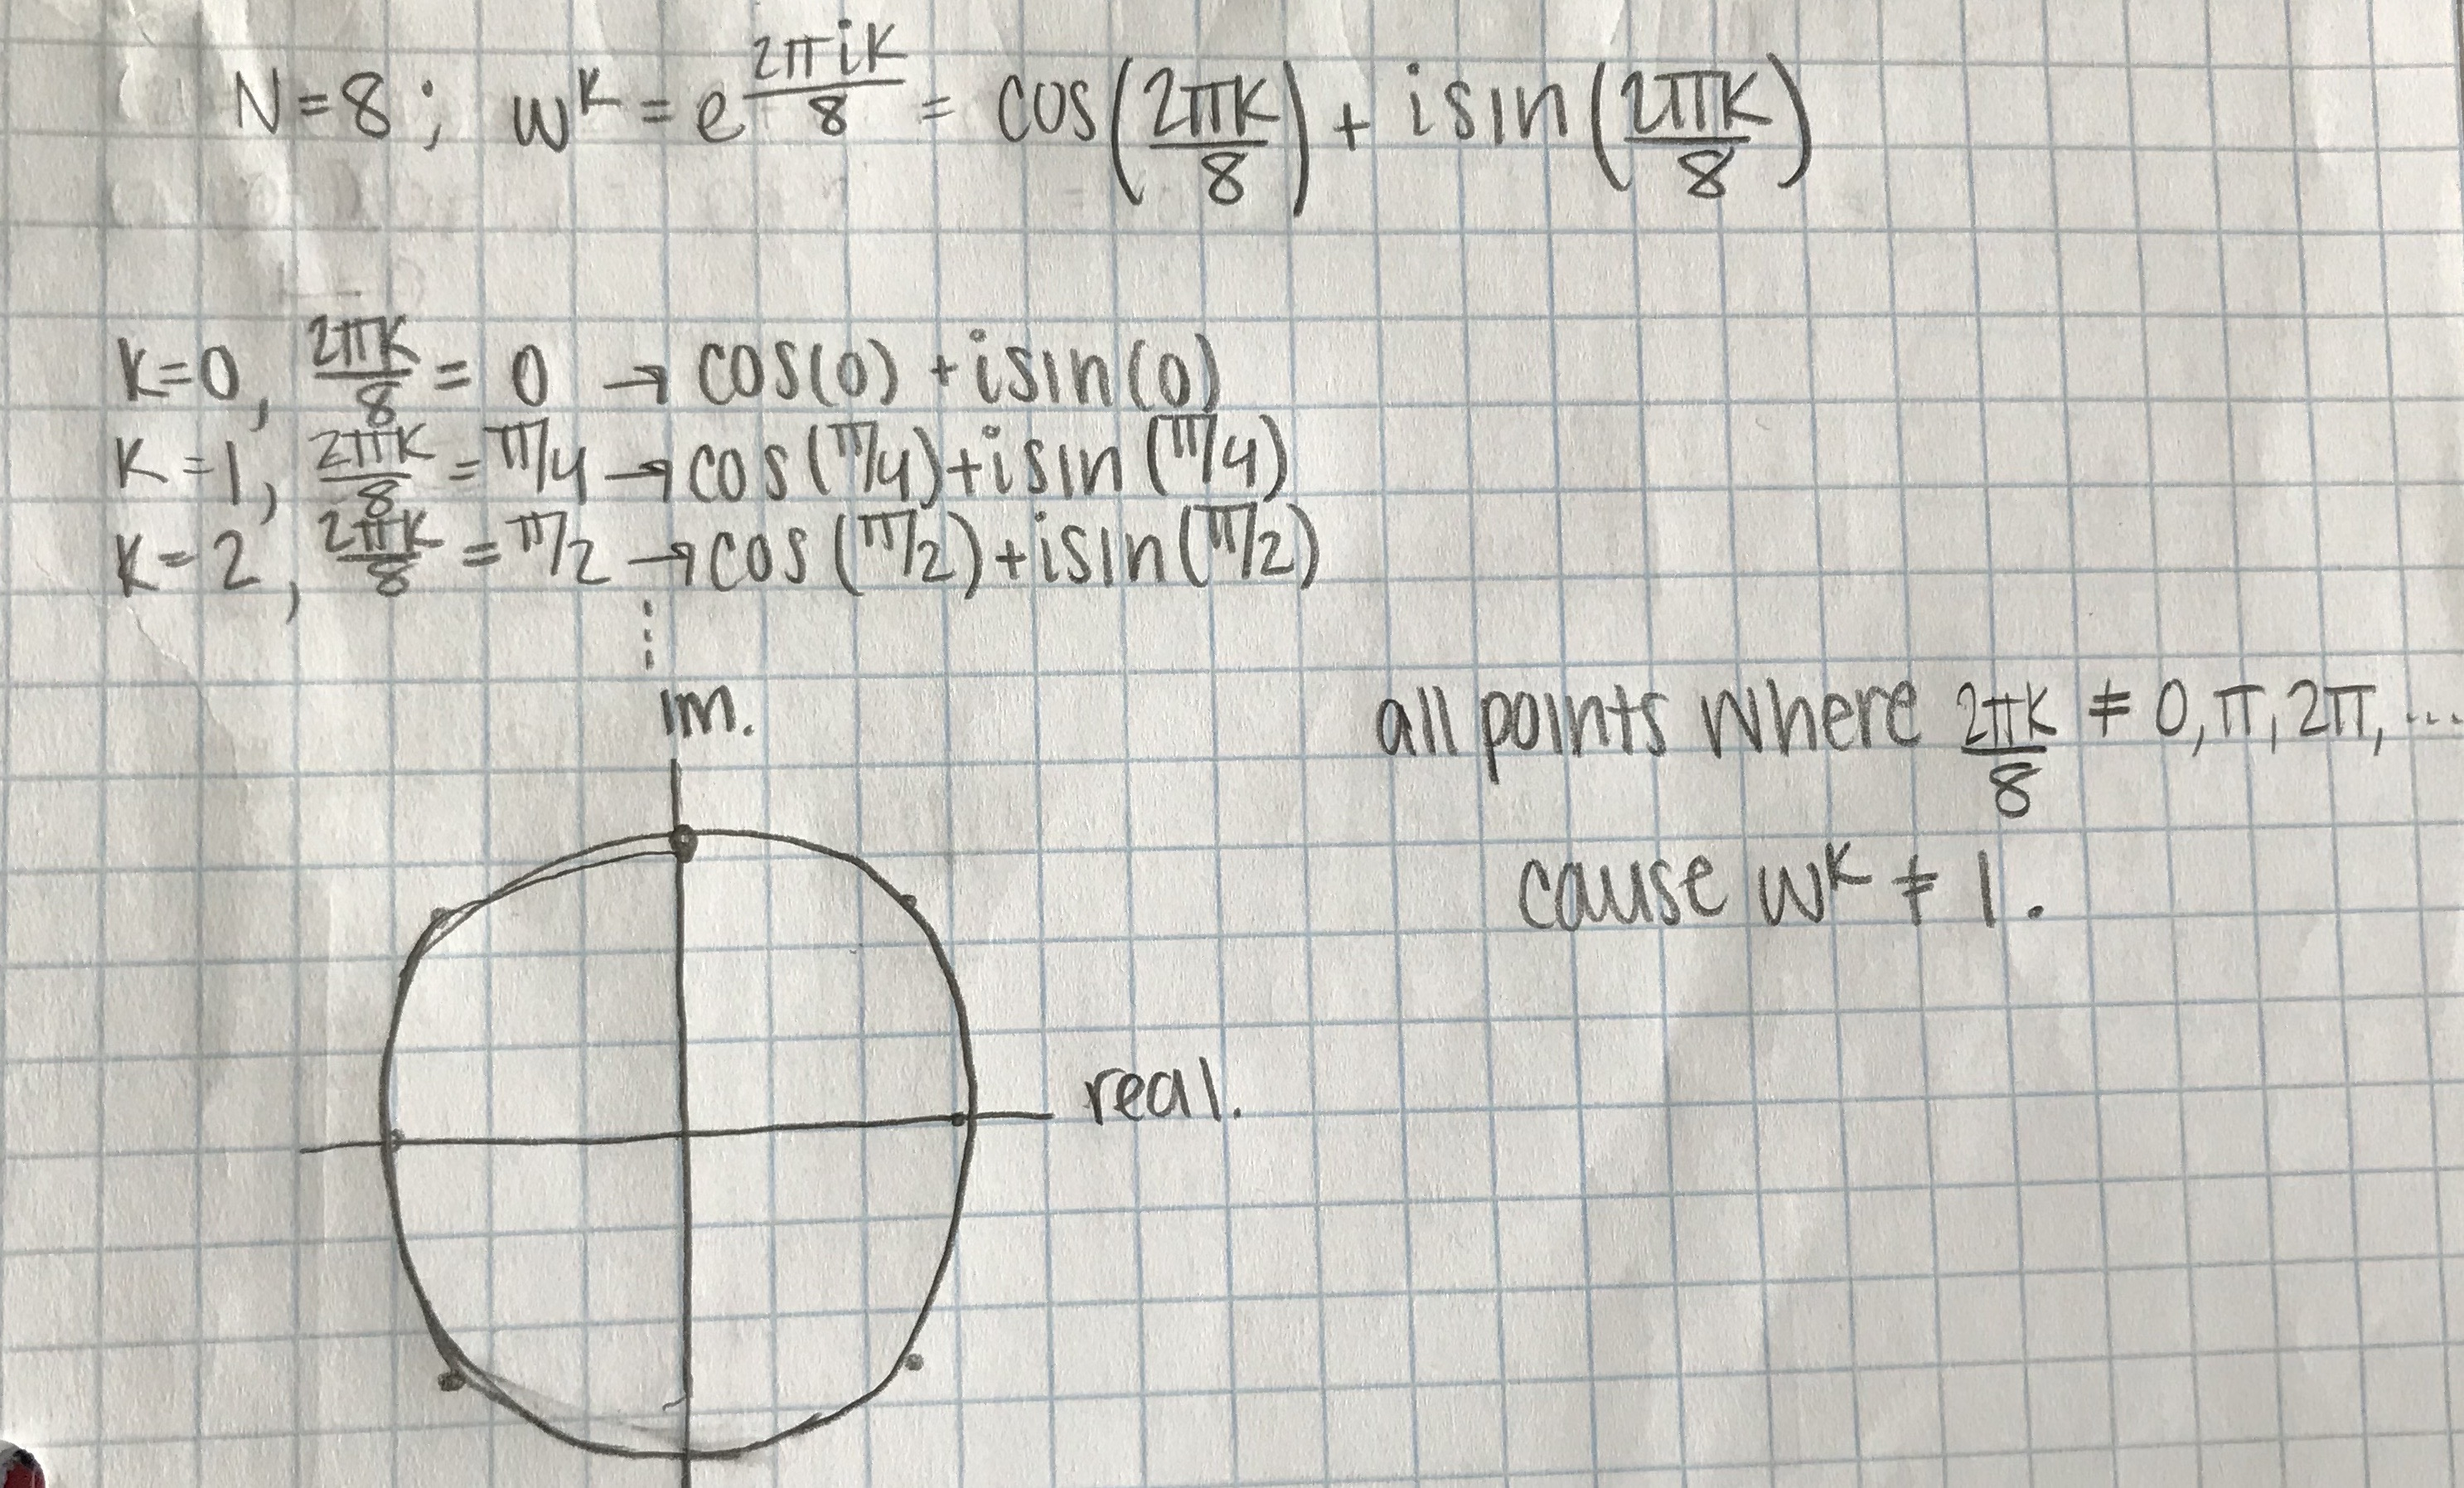
\includegraphics[scale=0.1]{exercise19} 

%exercise 20
\item 
\begin{eqnarray*}
	D^H &=& (\overline{D})^T\\
	D^HD &=& (\overline{D})^TD\\
	&=& NI
\end{eqnarray*}
because $D$ is an orthogonal matrix and $d_p \cdot d_q = N$ when $p=q$. 

%exercise 21
\item 
\begin{eqnarray*}
	D^{-1}D &=& \frac{1}{N}D^HD\\
	&=& \frac{1}{N} (NI) \mbox{    from above}\\
	&=& I
\end{eqnarray*}


%exercise 22
\item 63 $F_0, F_1, \dots$ values are printed out. $F_1$ and $F_63$ are the most significant. 

%exercise 23
\item Sine is attached to the imaginary spectrum and the only time this component is zero is when $\sin{(x)} = 0$, which is true when $x=0$. 

%exercise 24
\item $F_1, F_5$ and $F_59$ are the most significant.

%exercise 25
\item By setting two fo the significant values to zero, we got rid of the noise int he middle of the curve. 

%exercise 26
\item DFT can be used to solve partial differential equations. \url{https://www.math.kth.se/na/SF1538/projsim16/spectral_eng.pdf}

%exercise 27
\item $O(n^2)$

\end{enumerate}
\end{document}